\documentclass{beamer}

\usepackage[utf8]{inputenc}
\usepackage{pdfpc}
\usepackage{graphicx}
\usepackage{minted}
%Information to be included in the title page:
\title{Design and Implementation of a
Just-In-Time Compiler for Smalltalk}
\author{Fabian Lamprecht}
\date{16. Januar 2025}
\setbeamertemplate{navigation symbols}{}
\newcommand<>{\pnote}[1]{\only#2{\pdfpcnote{- #1}\relax}}

\begin{document}

\frame{\titlepage}

\begin{frame}
	\frametitle{Structure}
  \begin{itemize}
    \item Basics of Just-In-Time compilation
    \item Smalltalk-80
    \item Existing work
    \item Implementation details
	\end{itemize}
\end{frame}

\section{Just-In-Time compilation}

\begin{frame}
	\frametitle{Just-In-Time compilation}
  \begin{itemize}
		\item Goal: Fusing aspects of compiled and interpreted languages
    \item Compiled languages generally have a faster execution
    \item Interpreted languages are platform independant
    \item Just-In-Time is abbreviated as JIT
	\end{itemize}
\end{frame}

\begin{frame}
	\frametitle{How to build a JIT compiler}
  \begin{itemize}
    \item Interpreter as starting point
    \item compile every interpreted instruction to machine code 
    \item keep track of already compiled parts of the program
    \item add profiling to prevent compilation of rarely executed branches
    \item Program is split up in \textbf{Basic Blocks} (BB)
  \end{itemize}
\end{frame}

\begin{frame}
	\frametitle{Basic Blocks}
  \begin{itemize}
    \item start and end locations
    \item list of instructions 
    \item the generated machine code for this block
    \item heat value (see profiling)
    \item reference to the following BB
	\end{itemize}
  \pnote{More on how these work later in the Implementation details}
\end{frame}

\section{Smalltalk-80}

\begin{frame}
	\frametitle{Smalltalk-80}
  \begin{itemize}
    \item developed by, among others, Adele Goldberg and David Robson (Xerox PARC) 
    \item specified by the so called "Blue Book":  Smalltalk-80: the language and its implementation
    \item object oriented, variably typed (depends on the implementation)
    \item functionality resolves around message passing between objects/contexts
	\end{itemize}
\end{frame}

\begin{frame}
  \frametitle{Example of the execution of the addition of 3 and 4}

  \begin{figure}
    \begin{center}
      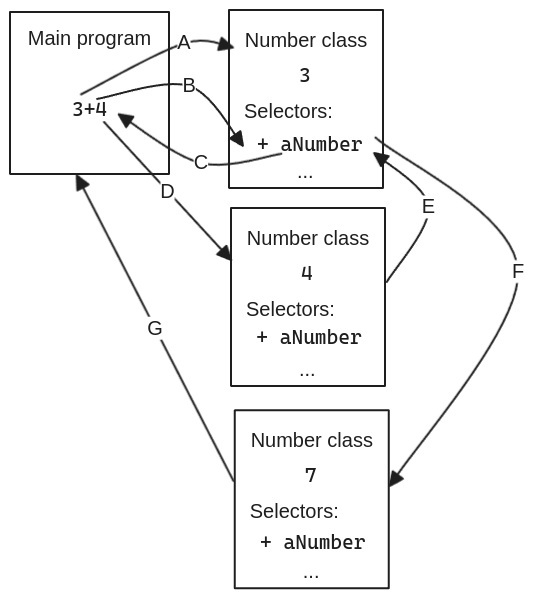
\includegraphics[width=0.5\textwidth]{../figures/illust3+4.png}
    \end{center}
  \end{figure}
  \pnote{A - Class lookup, B - Selector}
  \pnote{C - Selector return, D - Class lookup}
  \pnote{E - 4 is passed to the + selector, F - reference to 7 is created}
  \pnote{G - 7 is returned}
\end{frame}

\begin{frame}
  \frametitle{Smalltalk bytecodes}
  \begin{itemize}
    \item 29 instructions
    \item encoding ranges from 0 to 255 (8 Bit)
    \item may contain encoded parameters
    \item may require additional bytes as parameters
  \end{itemize}
\end{frame}

\begin{frame}
  \frametitle{Smalltalk bytecodes categories}
  These 29 Instructions can be categorized into 4 groups:
  \begin{itemize}
    \item Stack bytecodes
    \item Return bytecodes
    \item Send bytecodes
    \item jump bytecodes
  \end{itemize}
\end{frame}

\begin{frame}
  \frametitle{The Smalltalk-80 virtual machine}
  \begin{itemize}
    \item specified in the Blue Book
    \item abstraction layer to the real hardware
    \item constantly self evaluating
    \item parses the sourcecode to Smalltalk-80 bytecodes
  \end{itemize}
\end{frame}

\begin{frame}
  \frametitle{Terminology: Context}
  \begin{itemize}
    \item complete copy of the interpreter state at a point in time 
    \item maintains a seperate stack
    \item required for message sending (function calls)
    \item the interpreter has a pointer to the current context
  \end{itemize}
\end{frame}

\begin{frame}
  \frametitle{Terminology: Location}
  \begin{itemize}
    \item a position in the interpreted code 
    \item triplet of the pointers of the active context, the currently executed method and the method specific instruction pointer
  \end{itemize}
\end{frame}

\begin{frame}
  \frametitle{Terminology: Compiled Method}
  \begin{itemize}
    \item compiled representation of a method
    \item once a method gets interpreted successfully it is added to the interpreter as a valid receiver 
  \end{itemize}
\end{frame}

\begin{frame}
  \frametitle{Interpreter state}
  \begin{itemize}
    \item pointer to the compiled method 
    \item instruction pointer
    \item receiver and arguments of the message for the compiled method
    \item any temporary variables within the method
    \item the interpreter stack
  \end{itemize}
\end{frame}

\section{Existing work}

\begin{frame}
  \frametitle{Existing and related Work}
  \begin{itemize}[<+->]
    \item Dan Banays Smalltalk-80 interpreter 
    \item Rochus Kellers Smalltalk-80 interpreter
    \item LuaJIT based JIT compiler for Smalltalk-80 by Rochus Keller 
    \item Efficient Smalltalk by Deutsch and Schiffman
  \end{itemize}
\end{frame}

\section{Implementation details}

\begin{frame}
  \frametitle{Implementation of the Just-In-Time Compiler}
  \begin{itemize}
    \item Basis is a working Smalltalk-80 interpreter
    \item Injecting JIT specific code 
    \item Translation for each specific instruction into native machine code
  \end{itemize}
\end{frame}

\begin{frame}
  \frametitle{Implementation of the Just-In-Time Compiler}
  {\Huge \center Demo}

  \pnote{Start with interpreter loop, step through the logic, end at primitiveAdd}
  \pnote{Highlight Problems}
\end{frame}

\begin{frame}
  \frametitle{Conclusions}
  \begin{itemize}
    \item underestimated the complexity
    \item got stuck with insignificant details 
    \item general design seems solid enough to be a basis on further development
    \item project sparked interest in language design, compilers and interpreters as well as virtualization
  \end{itemize}
\end{frame}

\begin{frame}
  \frametitle{Future work}
  \begin{itemize}
    \item Expand on the existing solutions 
    \item verify the translation and correct execution of the machine code 
    \item verify the actual performance increase compared to the interpreters
  \end{itemize}
\end{frame}

\end{document}

